\subsection{Description du modèle}

Le modèle LNAS blé est une version plus complexe du modèle LNAS betterave. Le modèle est constitué de deux compartiments principaux : le compartiment circulation de biomasse et le compartiment simulation de l'eau. Dans cette section nous ferons une explication des principes généraux et une description qualitative du modèle. Le lecteur intéressé trouvera tous les détails en annexe dans  la référence que nous avons nous-même utilisé pour implémenter le modèle. \ref{ann:articlePierre}

\subsubsection{Circulation de biomasse}

\begin{figure}

\begin{center}
 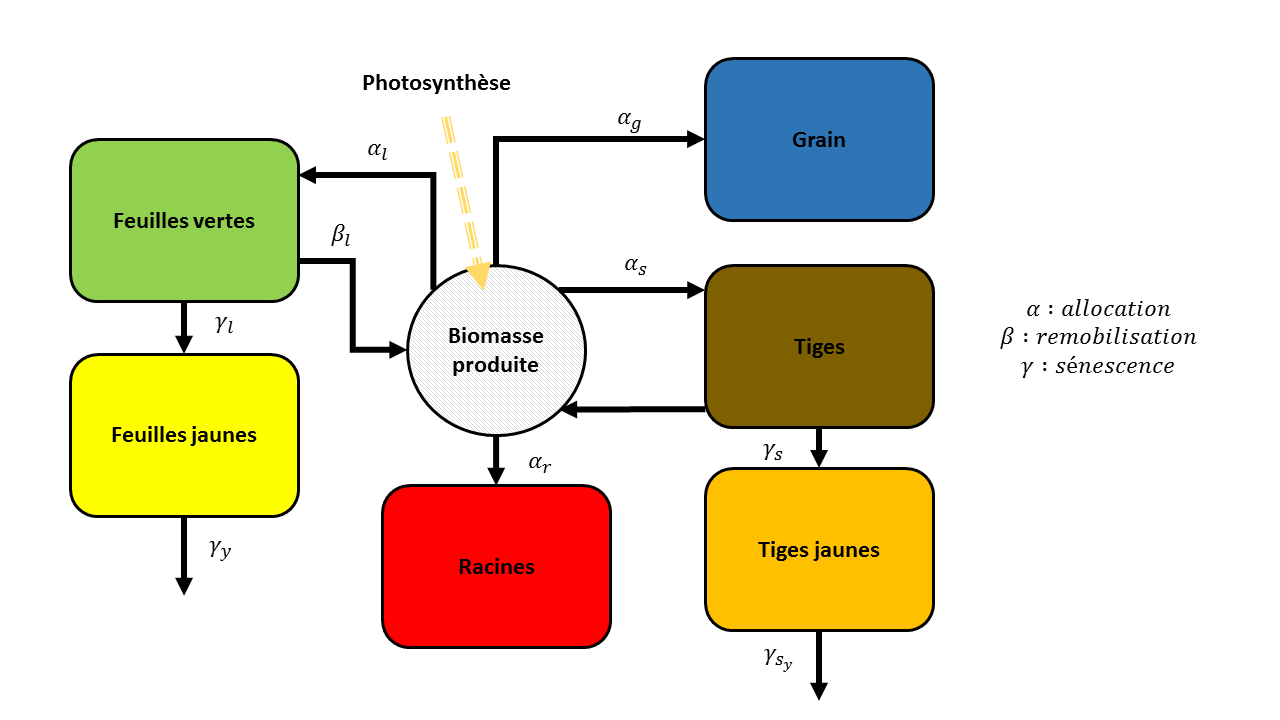
\includegraphics[scale = 0.7]{./img/modelSchema.png}
 \caption{Schéma de la circulation de biomasse}
 \label{fig:schemaModel}
\end{center}

\end{figure}

Le modèle va à chaque itération calculer la quantité de biomasse produite, l'ajouter à un pool de biomasse. Ensuite il va calculer des coefficients d'allocation, de remobilisation et de sénescence qui vont déterminer la circulation de biomasse entre les différents compartiment, la loi de conservation voulant que toute la biomasse soit allouée au final.

\begin{itemize}

\item La biomasse est produite par photosynthèse et la quantité crée est calculée grâce à la loi de Beer-Lambert.  Un coeffcient de stress hydrique et un coefficient de stress thermique peuvent réduire la production.

\item Des coefficient d'allocation sont ensuite calculés selon des lois log-normales, avec pour paramètres un temps caractéristique, à partir duquel l'allocation commence à être significative, une espérance et une variance. Typiquement, l'allocation aux racines et aux feuilles domine au départ, puis c'est celle aux tiges et vers la maturité de la plante c'est cella au grain.

\item Des coefficient de sénescence sont calculés selon des lois log-normales de la même façon. La sénescence des feuilles commence vers la fin de la croissance de la plante.

\item Enfin, des coefficient de remobilisation sont calculés toujours selon des lois log-normales. La remobilisation intervient de façon intense vers la fin pour les feuilles et les tiges en faveur du grain.

\end{itemize}

La valeur critique qui donne le rythme d'évolution de la plante n'est pas le temps réel mais le temps thermique qui correspond à l'accumulation de températures dépassant un certain seuil :
\[
\tau^{(n+1)} = \tau^{(n)} + \max[0, \underline{T^{(n)}} - T_c], 
\]
L'idée part d'un constat simple : la croissance de la plante est ralentie lorsque la température est basse.



\subsubsection{Simulation de l'eau}

\begin{figure}

\begin{center}
 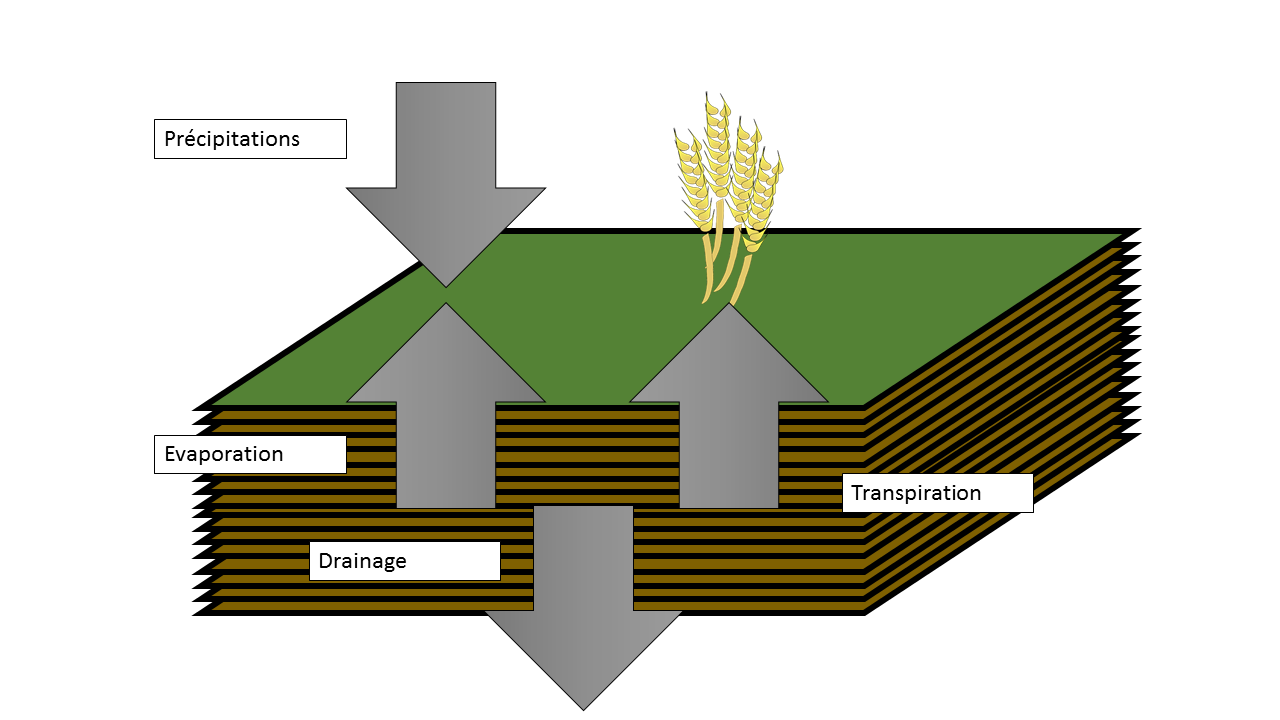
\includegraphics[scale = 0.7]{./img/waterSchema.png}
 \caption{Schéma de simulation de l'eau}
 \label{fig:waterModel}
\end{center}

\end{figure}

La simulation de l'eau est assez précisément décrit dans le modèle. 

Elle repose sur l'équation d'équilibre de l'eau
\[ {R^{(n+1)}}=R^{(n)}+W^{(n)}-Es^{(n)}-Tp{(n)}-d{(n)}\]

\[W^{(n)}\] représente les précipitations quotidiennes,\[Es^{(n)}\] est la quantité d'eau perdue par évaporation, \[Tp^{(n)}\] est la quantité d'eau transpirée par la plante et \[d^{(n)}\] est une fonction de drainage qui évacue l'eau ne pouvant être absorbé si le sol est saturé. 

On calcule l'évaporation et la transpiration potentielles, qui sont la quantité d'eau pouvant être évaporée et transpirée en fonction de l'environnement (evapotranspiration du milieu, ensoleillement...). 
Puis l'évaporation et la transpiration "max" qui sont celles requises étant donnée la plante et l'environnement (profondeur des racines, ensoleillement...). 
On regarde donc la transpiration et l'évaporation qui aura effectivement lieu, qui sera le minimum entre le potentiel et ce qui est demandé.
Si la transpiration requise pour la plante n'est pas satisfaite, il y aura un stress hydrique. 

Une fois l'évaporation et la transpiration déterminée on rajoute au sol l'eau apportée par les précipitations puis on enlève l'eau évaporée puis transpirée. Les apports et pertes d'eau se font en FIFO (First In, First Out) ou "piles" : l'eau est d'abord rajoutée sur les couches supérieures jusqu'à saturation à l'humidité maximale (humidité au delà de laquelle le sol ne peut plus absorber d'eau) avant d'être rajoutée aux couches les plus basses, de même, on retire l'eau des couches supérieures d'abord jusqu'à atteindre l'humidité minimale (humidité en deçà laquelle on ne peut plus tirer d'eau), avant de retirer l'eau des couches les plus basses.
Tout excès éventuel d'eau après opérations est drainé.